\documentclass[a4paper]{article}
\usepackage{pythonhighlight}
\usepackage[utf8]{inputenc}
\usepackage[T1]{fontenc}
\usepackage{textcomp}
\usepackage[dutch]{babel}
\usepackage{amsmath, amssymb}
\usepackage{code}
% figure support
\usepackage{import}
\usepackage{xifthen}
\pdfminorversion=7
\usepackage{pdfpages}
\usepackage{transparent}
\usepackage{graphicx}
\pdfsuppresswarningpagegroup=1
\graphicspath{{./img/}}
\begin{document}
    \section{Navigation Stack}
    \begin{itemize}
        \item set of ros nodes and algorithms used to make robot move autonomously
        \item takes input of 
            \begin{itemize}
                \item current location
                \item desired location
                \item odom data(wheel encoders,IMU,GPS) 
                \item laser scan (optional)
            \end{itemize}
        \item outputs velocuty commands \textbf{cmd\_vel}
        \item the nav stack is generic - can work with any moving robots
        \item works better with diff-drive and holonomic
        \item better with square and circular dhaped bots
    \end{itemize}
   \begin{figure}[h]
       \centering
       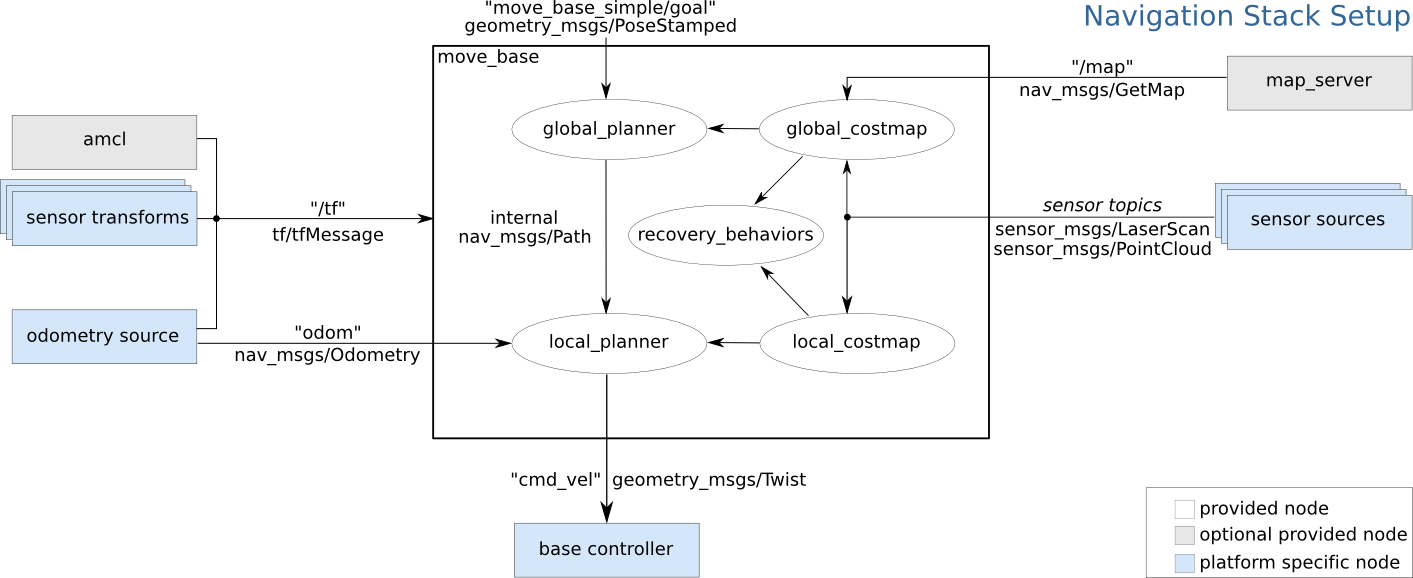
\includegraphics[width=0.8\textwidth]{./img/navstack-setup.png}
       \caption{nav stack setup}
       \label{fig:navstack}
   \end{figure} 
   explanation of the blocks in figure ~\ref{fig:navstack}
   \begin{itemize}
       \item \textbf{Odometery source} - current w.r.t to starting position. Main sources are wheel encoders,IMU,2d/3d cameras (visual odom) - [msg type : nav\_msg/Odometery]
       \item \textbf{sensor source } - localizing (laser scans) \& detecting obstacles (sonar,pcl)
       \item \textbf{sensor transforms} - each sensor must be refrenced with robots common frame(base\_link)
       \item \textbf{base\_controller}-converts nav stack msg to motor velocities
   \end{itemize}
\section{the move\_base}
\begin{itemize}
    \item most imp node in nav stack 
    \item moves the robot from current position to goal position with help of other nav nodes
    \item list of packages linked with move\_base
        \begin{itemize}
            \item global-planner
            \item local-planner
            \item rotate recovery 
            \item clear-costmap-recovery
            \item costmap-2D
        \end{itemize}
    \item other packages interfaced with mave\_base 
        \begin{itemize}
            \item map-server
            \item AMCL(adaptive monte-carlo localisation)
        \end{itemize}
    \item to summarise 
        \begin{figure}[h]
            \centering
            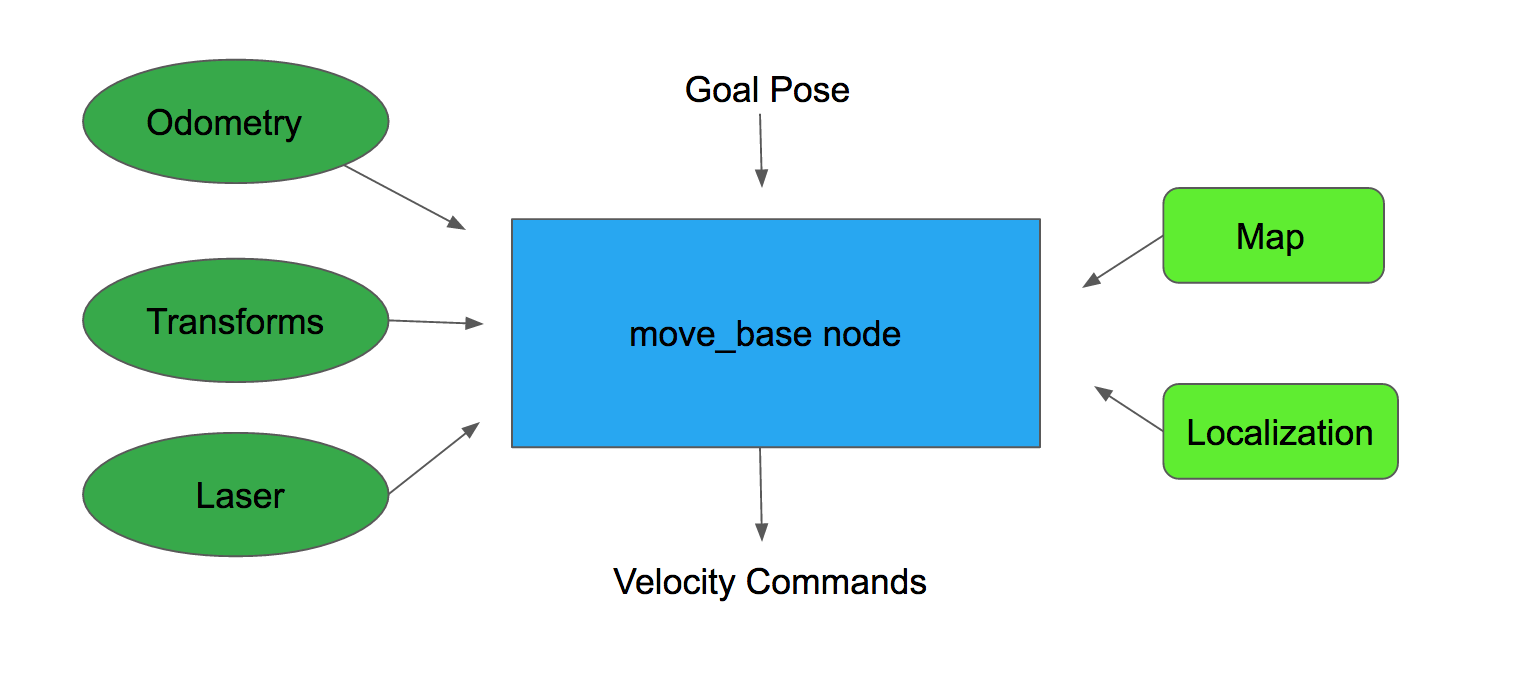
\includegraphics[width=0.8\textwidth]{./img/unit1-summary.png}
            \caption{}
            \label{fig:}
        \end{figure}
\end{itemize}

\end{document}
